\section{Interfaccia utente}
\subsection{Sezioni comuni}
Tutte le pagine dell'applicazione sono caratterizzate da un layout comune, che
include:
\begin{itemize}
    \item \textbf{Intestazione:} contiene il logo del progetto e il titolo dell'applicazione;
    \item \textbf{Contenuto principale:} è la sezione centrale della pagina, in cui viene visualizzato il contenuto specifico della pagina;
    \item \textbf{Piè di pagina:} contiene informazioni sul copyright e i link ai profili social del progetto;
\end{itemize}
\begin{figure}[ht!]
    \centering
    
\includegraphics[scale=0.6]{template/images/placeholder.png}
    \caption{Sezioni comuni}
\end{figure}

\subsection{Homepage}
La homepage è la prima schermata che l'utente visualizza all'apertura
dell'applicazione. L'elemento principale è un menu a tendina, situato al centro
della pagina: esso contiene una lista di dataset, ognuno dei quali rappresenta
un argomento di studio diverso. Scegliendo un'opzione dal menu, l'utente può
visualizzare le informazioni relative a quel dataset:
\begin{itemize}
    \item Nome del dataset;
    \item Breve descrizione del dataset;
    \item Dimensioni del dataset (numero di righe e colonne);
    \item Link all'ambiente 3D associato al dataset.
\end{itemize}
L'utente può espandere ciascun elemento della
lista per accedere a una vista dettagliata con maggiori informazioni. Una volta
selezionato un dataset, l'utente dovrà attendere il caricamento dei dati. Al
termine, verrà reindirizzato all'ambiente 3D.

\begin{figure}[ht!]
    \centering
    
\includegraphics[scale=0.6]{template/images/placeholder.png}
    \caption{Homepage}
\end{figure}

\subsection{Ambiente 3D}
L'ambiente 3D è la schermata principale in cui l'utente può visualizzare i dati
e interagire con essi.

\subsection{Grafico 3D}
Il grafico 3D è l'elemento centrale dell'ambiente 3D e rappresenta il dataset
selezionato. Ogni barra del grafico rappresenta un valore specifico del
dataset, mentre l'altezza della barra indica il valore stesso. Le barre sono
colorate in base al loro valore, con una scala di colori che va dal rosso
(valori bassi) al verde (valori alti). All’interno dell'ambiente 3D l'utente
può interagire con il grafico con le seguenti modalità:
\begin{itemize}
    \item \textbf{Spostamento:} l'utente può spostare il grafico senza cambiarne 
        l'angolazione tenendo premuto il tasto destro del mouse e trascinando 
        nella direzione desiderata;
    \item \textbf{Zoom:} l'utente può ingrandire o ridurre il grafico
        utilizzando la rotellina del mouse o il gesto di pinch sul touchpad;
    \item \textbf{Rotazione:} l'utente può ruotare il grafico senza spostarlo
        tenendo premuto il tasto sinistro del mouse e trascinando nella direzione desiderata;
    \item \textbf{Reset:} l'utente può riportare il grafico alla posizione 
        iniziale premendo il tasto "R" della tastiera.
\end{itemize}
Questi controlli sono sempre attivi quando il cursore è sopra il grafico.
\clearpage
\begin{figure}[ht!]
    \centering
    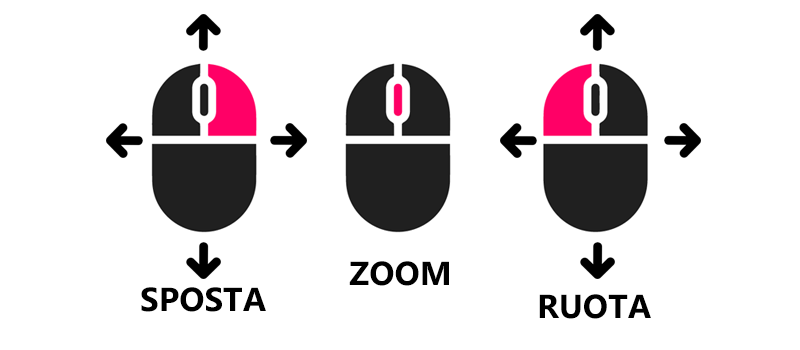
\includegraphics[scale=0.6]{template/images/comandi.png}
    \caption{Comandi per la navigazione}
\end{figure}

